\documentclass[12pt]{article}

% Language setting
% Replace `english' with e.g. `spanish' to change the document language
\usepackage[english]{babel}

% Set page size and margins
% Replace `letterpaper' with`a4paper' for UK/EU standard size
\usepackage[letterpaper,top=2cm,bottom=2cm,left=3cm,right=3cm,marginparwidth=1.75cm]{geometry}

% Useful packages
\usepackage{amsmath}
\usepackage{amsfonts}
\usepackage{graphicx}
\usepackage{setspace}
\usepackage{minted}
\usepackage{braket}
\usepackage{float}
\usepackage[colorlinks=true, allcolors=blue]{hyperref}
\usepackage{hypcap}
\usepackage{fancyhdr}

% xyqcirc stuff
\usepackage[frame,line,arrow,matrix,tips]{xy}	% all that is usually necessary

\doublespacing

\title{Quantum Bogosort}
\author{George Huebner}
\date{March 18, 2022}

\begin{document}
\pagenumbering{gobble}

\begin{titlepage}
\maketitle
\centering
\large Chicago STEM Fair, Computer Science Research, Design Category \\
\vspace{3em}
\huge Sponsor \\
\vspace{1em}
\large Michael Caines \hspace{15em}
\end{titlepage}

{
\hypersetup{hidelinks}
\tableofcontents
}
\pagebreak

\pagestyle{fancy}
\fancyhead[R]{\textit{Quantum Bogosort}, Huebner}
\fancyhead[L]{}

\pagenumbering{arabic}

\begin{abstract}
\noindent Gag algorithms are a staple of computer science and provide many a good chuckle. Take, for instance, MiracleSort\textsuperscript{\cite{thompson_2013}}, an algorithm that relies on alpha particle emission to cause erroneous bit flips to sort a list:
\begin{minted}{python}
while isSorted(unsorted_list) is False:
    time.sleep(1000)
\end{minted}
Despite their apparent uselessness, joke algorithms provide valuable insight into algorithm design and complexity\textsuperscript{\cite{gruber_holzer_ruepp_2007}}. In this paper we propose an implementation to Quantum Bogosort, one such joke algorithm.
\end{abstract}

\section{Introduction}

Classic Bogosort is a joke sorting algorithm where a list is randomly permuted and checked to see if it is sorted. Essentially, in pseudocode:

\begin{minted}{python}
while isSorted(unsorted_list) is False:
    random.shuffle(unsorted_list)
\end{minted}

\noindent It has an average time complexity of $ O((n+1)!) $ and the nondeterministic (traditional) method has an unbounded worst case time complexity for any non-trivial list.

Quantum Bogosort\textsuperscript{\cite{ryder_2018}}, then, is a variation on classical bogosort. Based on the \href{https://www.pbs.org/wgbh/nova/manyworlds/pdf/dissertation.pdf}{many worlds} interpretation of quantum mechanics, QBS proposes that a quantum computer can superimpose all possible permutations of a list and destroy any universe in which a sorted list does not exist, thus sorting the list in $ O(1) $ time. Because parallel universes are non-communicating, there's no way to know the list is sorted other than by the principle of quantum necessity. The algorithm that satisfies subscribers of the Copenhagen interpretation (where wave functions collapse) is essentially the same thing, but the quantum circuit must be run until the list is sorted.

Classical computers can already sort lists with a lower bound time complexity of $\Omega (N \log_2 N)$. Consequently, research into quantum sorting algorithms has been minimal, as the only optimizations possible are reducing space complexity. Because quantum computers do not have anywhere near enough qubits (let alone the error resilience) to realize this reduced complexity, sorting has been left to classical computers.

\section{Background}
Most people are likely unfamiliar with quantum computing and its associated quirks, so a minor detour is in order to explain the technologies that will be used to test the QBS algorithm. Explaining the quantum mechanics that underlie this project is well beyond the scope of a math symposium, though, so let the physics enthusiast proceed carefully.

\subsection{Quantum Computers}
Quantum computers should be thought of not as processors that parse instructions, but rather circuits composed of gates that operate on a group of qubits (\textbf{qu}antum \textbf{bit}, the quantum unit of information). While revolutionary, quantum computers only achieve speedups in certain applications, and have not yet cleared a benchmark of true quantum supremacy due to current hardware implementations. Current noisy intermediate scale quantum (NISQ) computers are highly error prone and have comparatively few qubits and are better thought of as a separate processing unit to be orchestrated by a classical computer.

\subsection{Qubits}
Qubits have quantum properties of superposition, entanglement, and interference that distinguish them from classical bits. Whereas a classical bit is either 1 or 0, a qubit is in a superposition of 1 and 0, which are defined as the following kets:
$$ \ket{0} = \begin{bmatrix} 1 \\ 0 \end{bmatrix} \text{ (Classical 0)} $$
$$ \ket{1} = \begin{bmatrix} 0 \\ 1 \end{bmatrix} \text{ (Classical 1)} $$
Qubit superpositon can be thought of as having a certain amount (amplitude) of 'one-ness' and 'zero-ness' that can be represented as so:
$$ \ket{x} = \alpha \ket{0} + \beta \ket{1} \ | \ \text{ Probability}_{\ket{0}} = | \alpha |^2 \text{, } \text{ Probability}_{\ket{1}} = | \beta |^2 $$
%Note that $|x|$ here represents magnitude as $\alpha$ and $\beta$ are imaginary.
To actually make use of qubits, they must be measured, which collapses them to either $\ket{0}$ or $\ket{1}$. This is a probabilistic, quantum event, hence the probability\textsubscript{$\ket{x}$}. It is helpful to consider the \hyperref[fig:bsphere]{Bloch sphere} when analyzing qubit state and rotation around the Pauli axes; essentially, the 'North Pole' is defined as $\ket{0}$ and the 'South Pole' is defined as $\ket{1}$. The 'equator,' then, would be an even superposition of $\ket{0}$ and $\ket{1}$.

\begin{figure}[H]
    \centering
    \capstart
    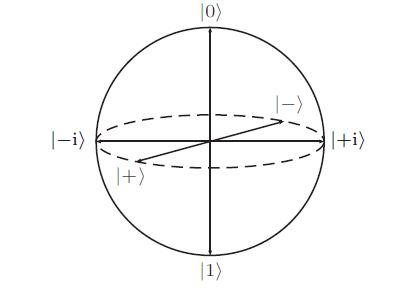
\includegraphics[width=0.3\textwidth]{images/bloch_sphere.png}
    \caption{Bloch sphere\textsuperscript{\cite{wikipedia_2021}}}
    \label{fig:bsphere}
\end{figure}

\noindent Here are a few common qubit gates:
$$ \text{X}(\ket{0}) = \ket{1} $$
$$ \text{X}(\ket{1}) = \ket{0} $$
$$ \text{Z}(\ket{0}) = \ket{0} $$
$$ \text{Z}(\ket{1}) = -\ket{1} $$
$$ \text{H} = \text{R}_{\text{y}} (\frac{\pi}{2}) \text{Z} \ \ \ \text{(Hadamard gate)}$$
$$ \text{H}(\ket{0}) = \frac{1}{\sqrt{2}} \ket{0} + \frac{1}{\sqrt{2}} \ket{1} = \ket{+} $$
$$ \text{H}(\ket{1}) = \frac{1}{\sqrt{2}} \ket{0} - \frac{1}{\sqrt{2}} \ket{1} = \ket{-} $$
Notice that R\textsubscript{y} is an arbitrary rotation around the Pauli Y-axis; Similarly, R\textsubscript{x} and R\textsubscript{z} allow arbitrary rotations along the X- and Z-axes, respectively.\\
Multiple qubits can be used together for entanglement and amplitude interference, and a group of qubits is called a \textit{register}. Although a register can be simplified into a single tensor by taking the tensor product of the qubits in the register, keeping registers in kets makes the math much simpler. \\
Bra-ket (Dirac) notation is used as Kronecker products quickly become unwieldy when dealing with large qubit registers.

\begin{figure}[h]
    \centering
    $$ \ket{x} \otimes \ket{y} = \begin{bmatrix} x_0 \\ .. \\ x_n \end{bmatrix} \otimes \begin{bmatrix} y_0 \\ .. \\ y_m \end{bmatrix} = \begin{bmatrix} x_0 \cdot \begin{bmatrix} y_0 \\ .. \\ y_m \end{bmatrix} \\ .. \\ x_n \cdot \begin{bmatrix} y_0 \\ .. \\ y_m \end{bmatrix} \end{bmatrix} = \ket{xy} $$
    \caption{Elegance of Bra-ket notation}
    \label{fig:my_label}
\end{figure}

\subsection{Entanglement}
Qubit gates can also be controlled if another qubit is $\ket{1}$ (similar to an 'if' clause in a classical programming language). This allows for multiple qubits to be entangled with each other, essentially tying the 'fate' of the qubits together so that they can no longer be thought of as individual qubits but rather a single system. Measuring one qubit will also collapse the other entangled qubits, even if they were never observed. A famous example of this is Schr\"odinger's cat. In this thought experiment, the quantum event of a radioactive substance decaying is entangled with the fate of the cat. If the cat dies, the radioactive substance must have decayed, and if the radioactive substance did not decay, the cat must be alive (or, at the very least, not killed by poison).

\section{Algorithm Design}
The implementation will be written using Qiskit, a Python framework for creating, running and simulating quantum circuits, and tested with the IBMQ Aer and Manila simulators.
Let us define the following:

\begin{itemize}
    \item A list of elements, $array$
    \item The length (cardinality) of this list, $l$
\end{itemize}

\noindent When we began designing this algorithm, two implementations were considered:
\begin{enumerate}
\item One approach would be to store the complete representation of the list in a qubit register. In Qiskit:
\begin{minted}{python}
array = [1, 2, 3]
size = 8
circuit = QuantumCircuit([QuantumRegister(size) for _ in range(len(array))])
\end{minted}
\textit{Note that Python numbers have dynamic size, but our 8-bit size would afford us an unsigned char, that is:}
$ x \in \mathbb{Z} \mid 0 \leq x < 256 $ \\
This clocks in at a respectable $ O(l \cdot s) $ space complexity, where $ s $ represents the size in bits of the data type in the list; While this method could potentially be useful in other quantum algorithms, this would essentially just transpose a classic algorithm onto a quantum circuit --- In the spirit of faithfully implementing QBS, we sought a more idiomatic quantum solution.
 
\item The other approach explored is essentially a quantum random number generator. Instead of storing the list, we create $ N = l! $ evenly balanced register states ($l!$ being the number of permutations of $array$). A set of states $ [0, N) \cap \mathbb{N} $ will be prepared, each with an even amplitude. Concisely:
    $$ \sum_{x=0}^{N-1} \frac{1}{\sqrt{N}} \ket{x_{BE}} $$
Note that the quantum register will always be represented in \href{https://en.wikipedia.org/wiki/Endianness}{big-endian}.

Because we're storing our number in binary, we want the power of 2 greater than or equal to $ l! $. This means we have $ O(\lceil \log_2 l! \rceil) $ space complexity, which seems scary at first. However, with present-day NISQ technology, this is significantly more favorable than $ O(l \cdot s) $ for any useful data type. Also keep in mind that because element size isn't a concern, any size element or even elements of different types could be stored in the list (as long as every type used can be compared to each other).

\begin{figure}[h]
    \centering
    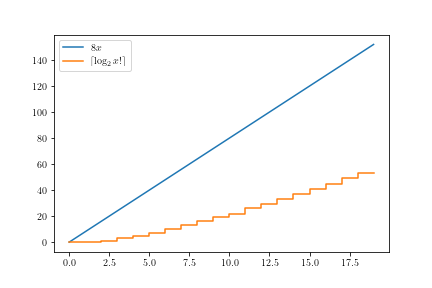
\includegraphics[width=0.54\textwidth]{images/size_compare.png}
    \caption{Space complexity comparison}
    \label{fig:chart1}
\end{figure}

Before we proceed, we would like to discuss the naive approach to quantum RNG. Applying H\textsubscript{ALL} (apply Hadamard to all qubits) to the entire register can create a number of superimposed states $ n $ such that $ n $ is a power of 2. We could still use this output to generate a random number $ h $ such that $ h \in [i, j] $:
$$ h = i + \frac{\text{M}(register)}{2^{|register|}} \cdot j $$
%Where $|register|$ is the cardinality of the qubit register. \\
The simplicity of this approach is actually not a bad thing: Because quantum computers suffer from high incidences of soft errors (such as erroneous qubit flips), reducing the complexity of a quantum circuit is ideal. Despite this, we wanted the challenge of implementing an algorithm that creates an even superposition of any number of states.
\end{enumerate}
 
\section{Quantum Bogosort}
\subsection{QRNG Algorithm}
The main algorithm is recursive, essentially moving through the register from most to least significant qubit, performing a R\textsubscript{y} gate to split up a qubit into P 'parts,' and entangling the remaining qubits with controlled Hadamard (CH) gates. \\
Let's use $i = 77$ as an example. Recall that for storing an integer $i$, the most significant bit (MSB) used is $\lfloor \log_2 i \rfloor$: For example, the MSB of 77 would be $\lfloor \log_2 77 \rfloor = 64$. Because QRNG generates the integers $[0, 77)$ (excluding 77 itself in order to generate 77 integers), we know that $[0, 64)$ is also being generated, because $[0, 64) \subseteq [0, 77)$. \\
This means that every possible state of the qubit register with a leading zero (in this case, in the 64s place) should be generated. That's already really easy to do! Just use the leading zero as a control and apply Hadamard gates to the rest of the register. Here's a simple example:
\begin{align*}
& \ket{\psi} = \ket{0000000} \\
& H(\psi_0), \ \ \ \ \ \ \ket{\psi} = \frac{1}{\sqrt{2}} \ket{0000000} + \frac{1}{\sqrt{2}} \ket{1000000} \\
& CH(\psi_0, \psi_{[1, 6]}), \ X(\psi_0), \ \ \ \ \ \ \ \ket{\psi} = \frac{1}{\sqrt{128}}(\ket{0000000} + \ket{0000001} + ... + \ket{0111111}) + \frac{1}{\sqrt{2}} \ket{1000000}
\end{align*}
Note that CH is a singly controlled Hadamard applied to multiple qubits, not a multi-controlled Hadamard applied to one qubit. Also note the X gate applied to the MSB because we really want an anti-controlled, not a normal controlled gate. \\
The problem is that we've unevenly split the integer 77 into 2: $|[0, 64)| \neq |[64, 77)|$. Numbers in the range $[64, 77)$ have a $(\frac{1}{\sqrt{13}} \cdot \frac{1}{\sqrt{2}})^2$ probability of being measured whereas numbers in the $[0, 64)$ range have a $(\frac{1}{\sqrt{64}} \cdot \frac{1}{\sqrt{2}})^2$ probability of being measured. \\
To fix this, we have to change the $\frac{1}{\sqrt{2}}$ from the Hadamard gate to something that gives us a more complex superposition; to do this we use the arbitrary rotation gates. $X$ and $Y$ gates give us the desired rotations we want, but we chose $Y$ so we don't have to worry about phase (the sign of a qubit). Phase doesn't matter in this case because only the magnitudes effect the probability of measurement, but it might be important if using QRNG in another algorithm. \\
Superpositions can be represented using spherical coordinates. For example, on the \hyperref[fig:bsphere2]{Bloch sphere}, the spherical coordinates $(1, 0.955, 0)$ would represent the state $\sqrt{\frac{1}{3}} \ket{0} + \sqrt{\frac{2}{3}} \ket{1}$ because $\cos (0.955) \approx \sqrt{\frac{1}{3}}$. We can do simple algebra to get a $\theta$ for an arbitrary superposition. For QRNG, this looks like $\theta = 2\arccos(\sqrt{\frac{77 - MSB}{77}})$. \\
\begin{figure}[H]
    \centering
    \capstart
    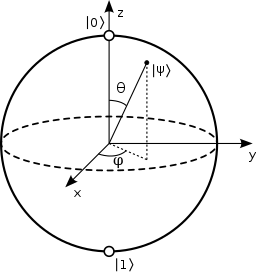
\includegraphics[width=0.19\textwidth]{images/bloch_sphere2.png}
    \caption{Bloch sphere\textsuperscript{\cite{wikipedia_2021}}}
    \label{fig:bsphere2}
\end{figure}
\noindent Recall that we have to apply a $X$ gate because gates are controlled by $\ket{1}$, not $\ket{0}$. We can save an extra gate by doubling our rotation (hence the 2), which gives us $\sqrt{\frac{77 - MSB}{77}} \ket{0}$ instead, which flips right back to $\ket{1}$ with another $X$ gate. \\
\indent We then recursively repeat this process, adding the MSB as a control qubit to the R\textsubscript{y} and CH gates and using the 2nd most significant bit as the new MSB. Eventually we split all the states evenly and we're done. \\

\noindent The differences between what is conceptually happening and what is actually implemented are shown below. $\bullet$ is a control and $\circ$ is an anti-control (controls on $\ket{0}$ instead of $\ket{1}$). Note that H\textsubscript{ALL} is \textbf{not} a multi-qubit gate --- it's illustrated that way for clarity.
\begin{figure}[H]
    \centering
    \includegraphics[width=0.9\textwidth]{images/circuits/conceptual_circuit.pdf}
    \caption{Conceptual circuit}
    \vspace{10mm}
    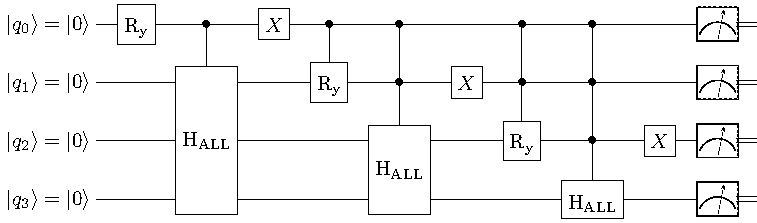
\includegraphics[width=\textwidth]{images/circuits/optimized_circuit.pdf}
    \caption{Circuit with proper controls}
    \label{fig:circs}
\end{figure}

\vspace{20mm}
\noindent Minor implementation details:
\begin{itemize}
    \item Multi-controlled Hadamard (MCH) gates are implemented manually with an ancilla qubit and multi-controlled X (MCX) gates. This could almost certainly be optimized more on a case-by-case basis (i.e. running \mintinline{python}{mode='noancilla'} for machines with fewer qubits).
    \item Especially when there are several qubits in the control register (and therefore the MCH gates are more costly), the MCX on the ancilla doesn't have to be reversed; instead, applying a  \mintinline{python}{'reset'} gate to reset the ancilla to 0 might be more optimal.
    \item \mintinline{python}{circuit} and \mintinline{python}{ancilla} don't change between recursions and needlessly add on to the stack frame of the function. Passing them as parameters is intended for clarity, but if you were to squeeze every drop of performance out they should be made global.
\end{itemize}
\subsubsection{Code}
\begin{minted}{python}
from qiskit import *
from math import acos, sqrt

def even_superpositon(circuit, register, controls, ancilla, P):
    if P <= pow(2, len(register)) / 2: # skip this iteration
        even_superpositon(circuit, register[1:], controls, ancilla, P)
        return
    if P == pow(2, len(register)): # reduced to H_ALL; base case
        if controls == []:
            for i in range(len(register)):
                circuit.h(register[i])
        elif len(register) > 0:
            circuit.mcx(controls, ancilla) # mcx to ancilla used in lieu of mch
            for i in range(len(register)):
                circuit.ch(ancilla, register[i])
            circuit.mcx(controls, ancilla)
        return


    extra_parts = P - pow(2, len(register) - 1)
    # this is the inverse of what we want, but saves us an X for ch
    theta = 2 * acos(sqrt(extra_parts / P))

    if controls == []:
        circuit.ry(theta, register[0])

        for i in range(1, len(register)):
            circuit.ch(register[0], register[i])
        controls += [register[0]]
    else:
        circuit.mcry(theta, controls, register[0])

        controls += [register[0]]
        circuit.mcx(controls + [], ancilla)
        for i in range(1, len(register)):
            circuit.ch(ancilla, register[i])
        circuit.mcx(controls, ancilla)

    circuit.x(register[0])

    even_superpositon(circuit, register[1:], controls, ancilla, extra_parts)
\end{minted}
\label{qrng}
\subsubsection{Testing}
Testing with an even superposition of 15 states:

\begin{minted}{python}
from math import ceil, log
from qiskit.visualization import plot_histogram

parts = 15
length = ceil(log(parts, 2))

register = QuantumRegister(length)
measurement = ClassicalRegister(length)
ancilla = QuantumRegister(1)
circuit = QuantumCircuit(register, ancilla, measurement)

even_superpositon(circuit, register, [], ancilla, parts)
circuit.measure(register, measurement)


count = execute(circuit, Aer.get_backend("aer_simulator"), shots=1024) //
.result().get_counts(circuit)
plot_histogram({key[::-1]: value for key, value in count.items()})
\end{minted}

\begin{figure}[h]
    \centering
    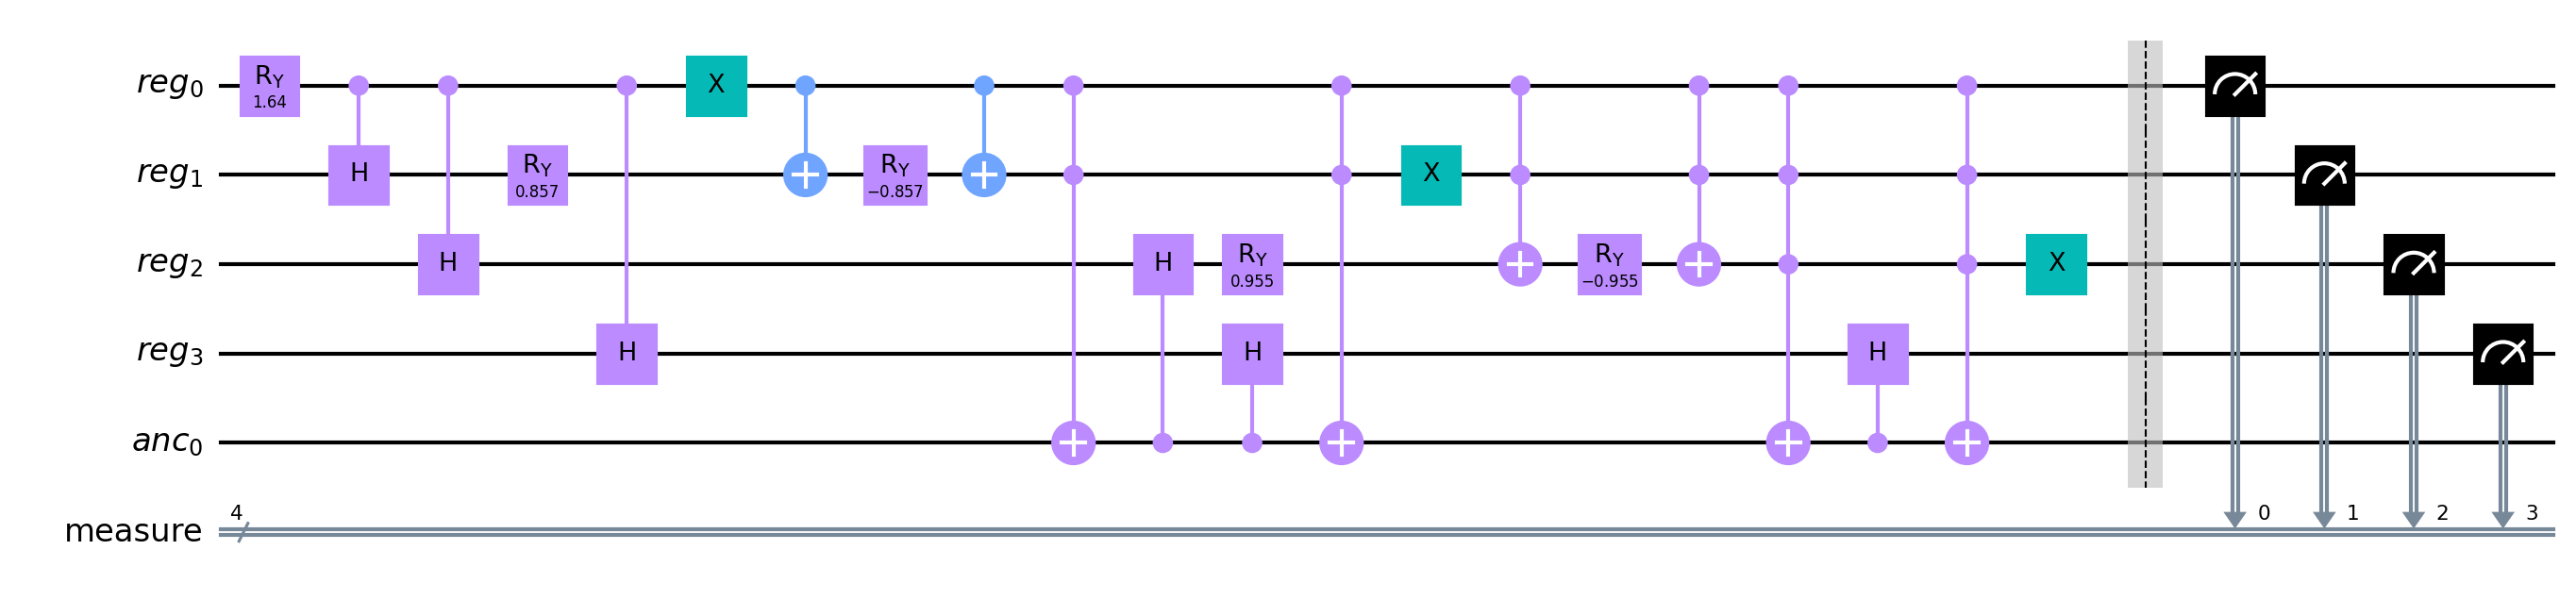
\includegraphics[width=\textwidth]{images/example_circuit.png}
    \caption{Circuit diagram for 15 'parts'}
\end{figure}
\begin{figure}[h]
    \centering
    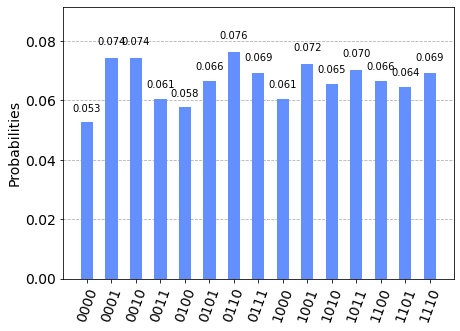
\includegraphics[width=0.75\textwidth]{images/example_measurement.png}
    \caption{Measurement results from Aer Simulator}
    \label{fig:measures}
\end{figure}

\subsection{Practicality Assessment}
Obviously bogosort is not meant to be a practical algorithm, but nevertheless we will conduct a review of the efficiency of QRNG.
\subsubsection{Time Complexity}
Although the original QBS proposal assumes the quantum circuit executes in $O(1)$ time, the depth (longest path) of the circuit does scale with input. The time a quantum circuit takes to execute is the sum of the gate execution times of the gates along the longest path of the circuit, and therefore time complexity scales with circuit depth. \\
For the integer $i$ passed into the QRNG algorithm, we allocate $\lceil \log_2 i \rceil + 1$ qubits. However, this algorithm is rather unique in that gate count and depth don't scale exactly with $i$, but rather \mintinline{python}{bin(i).count('1')}. That is, circuit depth scales with the number of ones in the binary representation of $i$. \\
Consequently, there are large drops in complexity around powers of 2:
\begin{align*}
&11111_2 \text{  (5 ones, high complexity)} \\ &+ 1 = 100000_2 \text{  (1 one, low complexity)}
\end{align*}
For example, $i = 256$ creates a circuit with depth 2 and width 17, but $i = 255$ has a circuit depth of 285 and a width of 17 (perhaps even more depending on transpilation target). This relationship is illustrated in \ref{fig:resources}.
% Also please note that depth + width $\geq$ total.

\begin{figure}[h]
    \centering
    \capstart
    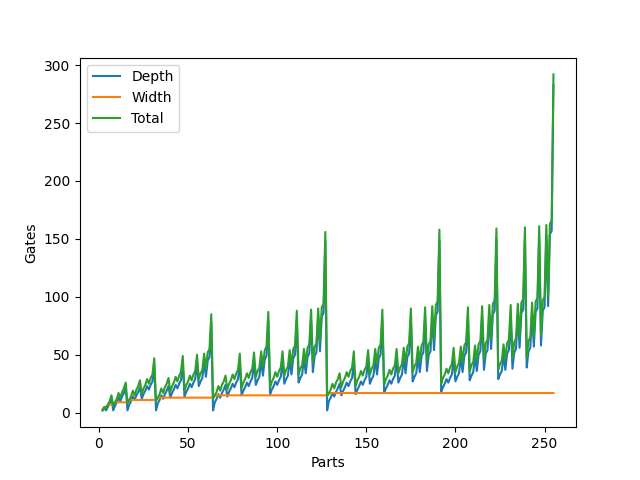
\includegraphics[width=0.9\textwidth]{images/resources.png}
    \caption{Circuit depth, width, and total gate count in relation to $i$}
    \label{fig:resources}
\end{figure}
\vspace{10mm}
\noindent With $o = $ \mintinline{python}{bin(n).count('1')}, we have a time complexity of $O(o)$ for many-worlds and $O(o \cdot n!)$ for Copenhagen.

\subsubsection{Error Rate}
Of course, the main problem with this ballooning circuit size is the fidelity of the measurement; we work with imperfect machines and error rates can compound over time to make a measurement meaningless. 
That being said, this is a QRNG algorithm, so the noise and error generated don't make much of a difference in this scenario (given that the noise is truly random and evenly distributed) besides occasionally measuring a number $ \geq i$. \\
We attempted to create a script to measure the error rate of a circuit based on IBMQ benchmarks, however this only measures the probability of every gate succeeding. This doesn't take into account several errors cancelling each other out or other fortuitous errors, and consequently the measured success rate is astronomically small. A good extension on this would be to use the error rates to modify each gate: For example, an $X$ gate with error $= 1.9765\mathrm{e}{-4}$ would translate to R\textsubscript{x}($(1-1.9765\mathrm{e}{-4}) \cdot \pi$). This would allow for the approximation of the expected position on the Bloch sphere during measurement, thus providing a more accurate error rate.

\subsection{Bogosort}
This is a fairly straightforward implementation of Quantum Bogosort:
\begin{enumerate}
    \item Generate all permutations of list with length $l$ (symbolic representations are fine to avoid memory overhead)
    \item Use QRNG with parts = $l!$
    \item Using the measured value from step 2, randomly select a permutation of the list
    \item If the permutation is sorted, return
    \item Repeat steps 1-4
\end{enumerate}
\vspace{15mm}
Note that with the many-worlds interpretation we can stop at step 4, because a universe where the list is sorted must exist (assuming the list can be sorted) by quantum necessity. Perhaps disappointingly, there's no destroying of universes in this algorithm.

\subsection{Complete Algorithm}
Using QRNG algorithm defined in \ref{qrng}
\begin{minted}{python}
from itertools import permutations
from time import perf_counter

def isSorted(ls):
    if not ls:
        return True

    prev = ls[0]
    for i in ls:
        if i < prev:
            return False
        prev = i
    return True

unsorted_list = [6, 10, 2589, 0, 47, 178, 324]
possibilities = list(permutations(unsorted_list))

parts = len(possibilities)
length = ceil(log(parts, 2))
register = QuantumRegister(length)
measurement = ClassicalRegister(length)
ancilla = QuantumRegister(1)
circuit = QuantumCircuit(register, ancilla, measurement)

even_superpositon(circuit, register, [], ancilla, parts)
circuit.measure(register, measurement)

start = perf_counter()
while True:
    counts = execute(circuit, Aer.get_backend("aer_simulator"), shots=500) //
    .result().get_counts(circuit)

    max_count = 0
    index = None
    for num, count in counts.items():
        if count > max_count and (benum := int(num[::-1], 2)) < parts:
            max_count = count
            index = benum

    if index is not None:
        if isSorted(possibilities[index]):
            break
end = perf_counter()

print(f"Finished Quantum Bogosort in {end-start} seconds on list of length //
      {len(unsorted_list)}")
\end{minted}
An impressive sort time of 258.02 seconds on a 7 element list... Quite bogus, indeed.

\section{Conclusion}
In this paper, we implemented the quantum bogosort algorithm using QRNG to randomly permute a list and check if it's sorted. Although QBS is a joke, the QRNG algorithm implemented could probably be useful in setting states where an H\textsubscript{ALL} wouldn't do the trick. Despite the fact that we couldn't find a similar QRNG algorithm, this seems too useful to be novel. \\
The QRNG algorithm presented could be further studied and improved for efficient preparation of arbitrarily superimposed qubits. Right now, QRNG generates an interval of integers, but this could be extended to generating an even superposition of arbitrary values. Additionally, as discussed in the practicality assessment, this algorithm does not scale well due to the prevalence of multi-controlled gates. \\
Another way to improve QBS would be to study how the list is sorted. Because the (non-unique) permutations of a list grows at $n!$, QRNG's $O(\log_2 n)$ space complexity quickly becomes overwhelmed with larger lists. Finding ways to reduce this inefficiency would be ideal, perhaps by using a 'divide and conquer' strategy (\`{a} la quicksort); However, this would defeat the purpose of bogosort! \\
We were able to both exercise previous knowledge of quantum computing and learn new skills in data collection and presentation. Additionally, we spent more time designing this algorithm because there's no previous implementation of QBS to compare against: Consequently we got to pursue many different solutions and choose the most interesting one. \\

\vspace{10mm}
\noindent All code was written and tested with Qiskit 0.32.0 \& Python 3.8 on WSL2 Ubuntu 20.04.1.

\vspace{15mm}
\noindent \emph{We acknowledge the use of IBM Quantum services for this work. The views expressed are those of the authors, and do not reflect the official policy or position of IBM or the IBM Quantum team.\textsuperscript{\cite{ibm_21}}}

\bibliographystyle{ieeetr}
\nocite{*}
\bibliography{sources}

\end{document}